\section{Introduction}
\label{sec:intro}
% \KZ{Cut this to 1.5 pages at most.}
% We focus on word+entity+verb distractors
Cloze-style multiple choice question (MCQ) is a common form of exercise used to evaluate the proficiency of language learners, frequently showing up
in homework, exams and official tests.
Figure \ref{fig:mcq} shows a cloze-style MCQ, which typically 
consists of: a question stem with a blank to be filled in, 
the correct answer and multiple wrong answers used to distract testees.
Despite the high demand, manual crafting of such MCQs is very time-consuming 
for educators, which calls for the automatic generation of 
practice material for students from readily available plain texts.
% Recently, automatic cloze-style MCQ generation has shown its potential in tasks such as English proficiency tests~\cite{sumita2005measuring}, vocabulary exams~\cite{susanti2018automatic}, knowledge assessments~\cite{guo2016questimator}. 
\begin{figure}[!htb]
	\centering
	\scalebox{1.0}{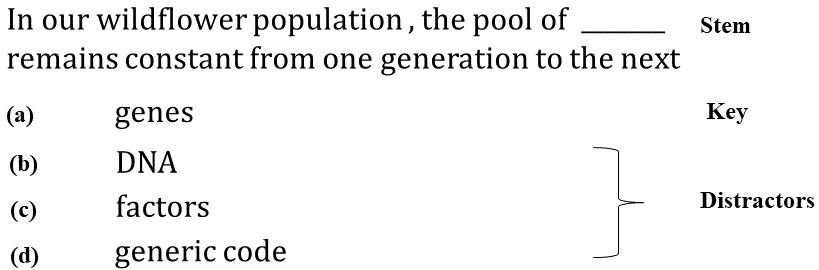
\includegraphics[width=1.0\columnwidth]{figure/mcq.jpg}}
	\caption{A Cloze-style MCQ} \label{fig:mcq}
	\end{figure}

% \KZ{Are these auto-generated MCQs for human or for machine to
% consume. Can auto-gen MCQs really replace human crafted questions? You need to picture the
% scenario a bit more to motivate the necessity of the problem because it's a niche domain.} 
Distractor generation (DG), which aims to generate distractive alternatives~(i.e., distractors) of the correct answer given the question stem, is a critical part of cloze-style MCQ construction. However, it is not only time-consuming but also non-trivial to come up with appropriate distractors without rich experience in language education.
% the quality of a MCQ relies heavily on the quality of these distractors~\cite{rodriguez2005three,haladyna2002review}. Good distractors ensure that the outcome of MCQ tests provides more credible and objective picture of the knowledge of the testees involved~(e.g.~Testees have to use expert knowledge in biology to distinguish that \textit{DNA} in Figure \ref{fig:mcq} is incorrect despite it is similar to \textit{genes}, and therefore \textit{DNA} is a good distractor). On the other hand, even beginners can easily identify that \textit{factors} is incorrectness since it is not semantically similar to \textit{genes} at all, making it a bad distractor. \textit{generic code} is also an correct answer, and therefore is an invalid distractor.
Literature in language pedagogy~\cite{haladyna2002review,pho2014multiple} generally recommonds two criteria for designing distractors: 
{\em plausibility} and {\em reliability}. 
By plausibility, it means distractors should be semantically related to 
the key and grammatically consistent with the context given by stem 
to adequately discriminate learners' proficiency. 
By reliability, it means the distractor, when filled into the blank of
the stem, results in a logically incorrect or inconsistent statement.

% issue 1. 词库太小了, domain-specific
% issue 2. 很少有把若干个metric similarity, shape score结合起来的模型。 
%learning to rank 可以,但vocabulary太小,没有考虑 reliability
% issue 3. 大多数方法没有考虑context 比如:Chinese fill-in 和 thearus-based method虽然考虑了reliability, 没有考虑 context 
Automatically generating distractors has been previously explored as part of cloze-style MCQ construction in a few studies. However, those methods generally assume advance knowledge of a specific domain~(e.g., science) of 
the given question and then use corresponding domain-specific vocabulary 
as candidate distractor set to rank based on using various unsupervised 
similarity heuristics~\cite{sumita2005measuring,Kumar2015RevUP,jiang2017distractor} or supervised machine learning model~\cite{sakaguchi2013discriminative,welbl2017crowdsourcing,liang2018distractor}.
Since identifying the concrete domain of each question and 
preparing large-scale domain-specific vocabulary require 
substantial human labor, such corpus-based methods cannot be easily 
applied in real-world scenarios.

% mostly based on various similarity measures, including embedding-based similarities~\cite{Kumar2015RevUP, guo2016questimator}, n-gram co-occurrence likelihood~\cite{hill2016automatic}, lexical similarities~\cite{pino2008selection}, thesaurus-based similarity~\cite{sumita2005measuring} and syntactic similarity~\cite{chen-etal-2006-fast}. Distractors are then selected using a weighted combination of above-mentioned similarities, where the weights are determined by human-crafted heuristics.

% \KZ{Existing work has the following issues: problem definition may not be practical, 
% dataset is narrow and not cross domain, or too small.}
% In contrast to the similarity-based line of work, \citet{liang2018distractor} formulate DG as a point-wise ranking problem by integrating previously proposed similarity measures and developed both feature-based ranking models and generative adversarial nets~\cite{liang2017distractor} that learn to select distractors automatically.  They achieve the state-of-the-art performance with feature-based ranking models. 
% Despite Liang et al.~\shortcite{liang2018distractor}'s success, they select distractors from a rather small vocabulary containing instances from SciQ~\cite{welbl2017crowdsourcing} and MCQL~\cite{liang2018distractor} datasets, which is not generalizable. Although there exist other candidate sources including ontology~\cite{stasaski2017multiple}, manually annotated corpora~\cite{zesch2014automatic,sakaguchi2013discriminative}, and thesaurus~\cite{sakaguchi2013discriminative}, they are all domain-specific and often limited in their coverage. To address this issue, some researchers~\cite{jiang2017distractor} propose to use words extracted from the Wiki corpus as distractor candidates. However, their method does not take the question context, an indispensable factor, into consideration. Whereas in this paper, our goal is to propose an open-domain context-dependent concept distractor generation framework. 
% Despite their success, they only implement the ranking model as a binary classifier and select distractors from a rather small vocabulary containing instances from SciQ~\cite{welbl2017crowdsourcing} and MCQL~\cite{liang2018distractor} datasets, which is not generalizable enough to cover distractors in open domain.

Another issue is that previous approaches mainly focus on selecting plausible distractors while rarely adopt reliability checks to ensure that the generated 
distractors are logically incorrect. 
Despite some attempts in early approaches~\cite{sumita2005measuring, jiang2017distractor}, 
they both used it in the post-processing step to filter out candidate 
distractors rejected by diverse predefined filters, which is sometimes 
too strict as it may exclude useful distractors like \textit{DNA} in 
Figure \ref{fig:mcq}.

% Moreover, another issue is that many previous work only focus on how to select plausible distractors, and adopt no or weak reliability checking, which is a critical part to ensure there is only one correct answer in each item.
% Although Sumita et al.~\shortcite{sumita2005measuring} conduct reliable checking based on retrieval from the Web, their hypothesis that an instance is a correct answer if it appears in search results of the stem is too strict. For the example in Figure \ref{fig:mcq}, \textit{DNA} is rejected by their reliable checking filter since it often appears together with \textit{genes} in web pages, but it is a very good distractor.

%简要介绍方法的亮点,需要和contribution对应
% \XZ{Briefly introduce how to fix these problems(two), show results and strengths of our methods}
In this paper, we propose a configurable distractor generation framework for English cloze-style MCQ in open domain, whose design is motivated by the shortcomings identified above. It mainly consists of two components: 
(1) a \textit{context-dependent} candidate set generator, which constructs a small set of 
candidate distractors from a general-purpose knowledge base, 
based on contextual information formed by the stem and the key; 
(2) a learning-to-rank model which takes both reliability checking and plausibility measures into consideration. By incorporating structured, human-curated
general-purpose knowledge base and conducting context-dependent 
conceptualization on the answer, we are able to effectively extract 
semantically-related candidate distractors without the need of 
domain-specific vocabulary. These candidate distractors are further re-ordered 
by a ranking model, trained with elaborately designed features to 
automatically control the trade-off between plausibility and reliability.

%To overcome these shortcomings, we propose an open-domain, data-driven framework for generating word distractors that are both plausible and reliable with contextual fit. Based on contextual information, We construct a small-size candidate set from a large-scale general-purpose knowledge source, Probase, which is constructed from billions of web pages. Since this candidate source is generalizable and diverse enough, our method is adoptable in different domains. While generating distractors, we are actually making a trade-off between plausibility and reliability, so we can not consider than them individually. Instead of conducting candidate filtering~\cite{jiang2017distractor}, we integrate new reliable checking features with other plausibility measures into distractor selector. 
% Our reliable checking features evaluates the correctness of (argument1, relation, argument2) triples extracted from the full sentence formed by the stem and a candidate and the collocations involving the candidate. 

%With these methods, our framework generates \textit{antigens, DNA, viruses} for the example in Figure \ref{fig:mcq} whose quality is comparable with \textit{DNA, eggs, genomes} designed by human experts. 
Previous DG methods~\cite{sumita2005measuring,agarwal2011automatic, Kumar2015RevUP,liang2017distractor,liang2018distractor} are evaluated either with sole human annotation or on ad hoc datasets that are often narrow in domain.
To the best of our knowledge, there is no open-source benchmark dataset for DG that is diverse enough to comprehensively evaluate the model performance. We construct a cross-domain cloze-style MCQ dataset~\footnote{\url{https://anonymous_for_blind_review}} covering science, trivia, vocabulary and common sense, which can be used as a benchmark for future research in DG. We further
investigated various instantiations of proposed framework. 
%Experimental results of both automatic and human evaluation show that our proposed framework achieves significant and 
%consistent improvement compared to several competing baselines.

The contributions of this paper are three-folds:
\begin{itemize}
	\item we compile and open-source presently the most diverse and comprehensive benchmark dataset for training and evaluating distractor generation model~(\secref{sec:data}).
	\item we propose a novel configurable distractor generation framework for open-domain cloze-style MCQ, which requires no domain-specific vocabulary and jointly evaluates the plausibility and reliability of distractors (\secref{sec:method}).
	\item we conduct comprehensive experiments to evaluate and analyze various instantiations of our framework and show that it consistently outperforms previous methods in both automatic ranking measures~(about 2\% F1 score) and human evaluation~(\secref{sec:endtoend}).
\end{itemize}
